\documentclass{mm2}
\usepackage{bbm}
\usepackage{bbold}
%\usepackage{float}
% REF: https://farside.ph.utexas.edu/teaching/336L/Fluid/node135.html
% http://galileo.phys.virginia.edu/classes/152.mf1i.spring02/RiverViscosity.pdf

\newcommand{\pdiff}[2]{\frac{\partial #1}{\partial #2}}
\newcommand{\pddiff}[2]{\frac{\partial^2 #1}{\partial #2^2}}


\cisid{dma0bmp} % retplace with your own
\title{Your Title}
\begin{document}

\begin{abstract}
  Your Abstract.
\end{abstract}



\section{Introduction}
Your Introduction

\section{A section}

Example of an equation
\begin{equation}
\delta N_i(t) = k(N_{i-1}(t)+N_{i+1}(t)-2N_i(t)), \qquad i=0\, \dots\, n-1 .
  \label{eq_diff_deltaN} % a usefull equation label
\end{equation}

We can refer to that equation using (\ref{eq_diff_deltaN})

\vspace{5mm}
\begin{answer}{1}
  This will be you answer to problem 1, but move this where appropriate.
\end{answer}

You should also add some text outside the answer to questions of course.

\vspace{5mm}
\begin{answer}{7}
  This will be you answer to problem 7, but move this where appropriate.
\end{answer}

The questions do not need to be answered in the numerical order.
\vspace{5mm}
\begin{answer}{8}
  This will be you answer to problem 8, but move this where appropriate.
\end{answer}

\begin{answer}{9}
  This will be you answer to problem 9, but move this where appropriate.
\end{answer}


The model equation
\begin{equation}
  \label{eq_chemo_disc}                           
  \begin{aligned}
  \frac{{\rm d}b_i}{{\rm d}t} &= \frac{1}{{\rm d}x}\left(\chi(b_{i-1},c_{i-1})\,b_{i-1}\,\frac{(c_{i}-c_{i-1})}{{\rm d}x}- \chi(b_i,c_i)\,b_i\,\frac{(c_{i+1}-c_{i})}{{\rm d}x}\right)\\[1ex]
                  &\equiv -\pdiff{}{x}\left(\chi(b,c)\, b\,
  \pdiff{c}{x}\right)
  \end{aligned}
\end{equation}


\vspace{5mm}
\begin{answer}{9}
  This will be you answer to problem 9, but move this where appropriate.
\end{answer}


This is how we include a figure

\begin{figure}[h]
  \begin{center}
  
\includegraphics[width=.5\textwidth]{Fig1.pdf}
  \caption{A figure description
  \label{fig_one} % label to reference the figure
  }
  \end{center}
\end{figure}

In figure \ref{fig_one} we can't see anything interesting yet.
An appropriate figure is needed!


We can also put several figures together
\begin{figure}[h]
  \begin{center}
  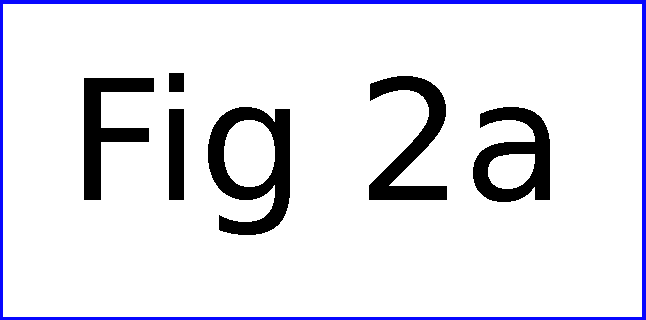
\includegraphics[width=.32\textwidth]{Fig2a.pdf}
  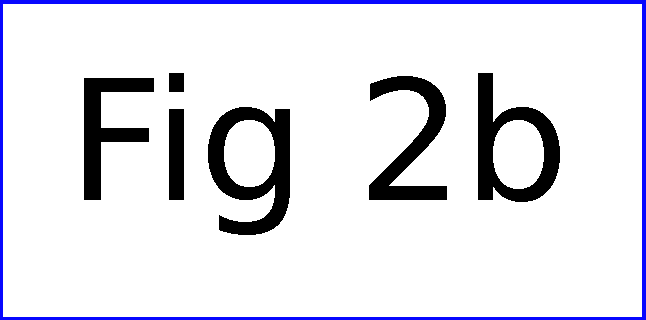
\includegraphics[width=.32\textwidth]{Fig2b.pdf}
  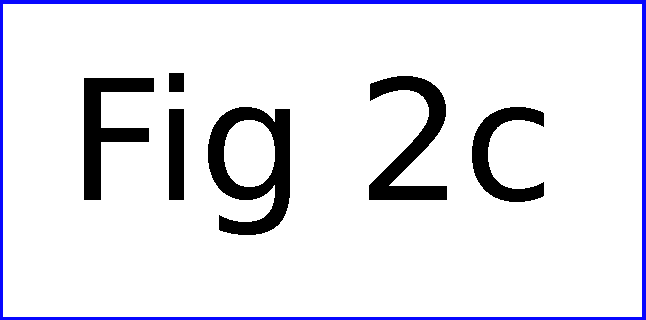
\includegraphics[width=.32\textwidth]{Fig2c.pdf}
  \break
  (a)\hspace{33mm} (b) \hspace{33mm} (c)
  \caption{Example of figures
    \label{fig_two} % label to reference the figure
  }
  \end{center}
\end{figure}



\section{Conclusions}
Your conclusions

The references: do you have any others.

\begin{thebibliography}{99}

\bibitem{Tindall}
M. J. Tindall, P. K. Maini, S. L. Porter, J. P. Armitage",
{\it Overview of Mathematical Approaches Used to Model Bacterial Chemotaxis II: Bacterial Populations}", Bull. Math. Biol.", (2008) 70, 1570.
\url{https://doi.org/10.1007/s11538-008-9322-5}


\bibliographystyle{plain}
\end{thebibliography}{}
\end{document}
